\documentclass[10pt,twocolumn,letterpaper]{article}

\usepackage{cvpr}
\usepackage{times}
\usepackage{epsfig}
\usepackage{graphicx}
\usepackage{amsmath}
\usepackage{amssymb}

% Include other packages here, before hyperref.
\usepackage{multirow}
\usepackage{psfrag}
\usepackage[ruled,vlined]{algorithm2e}
\usepackage{array}
\usepackage{forloop}
%% editing comment
\newcommand{\ignore}[1]{}   % ignore this
\newcommand{\cmt}[1]{\begin{sloppypar}\large\textcolor{red}{#1}\end{sloppypar}}

\newcommand{\todo}[1]{ \textcolor{red}{[{\bf TODO}: #1]}}
\newcommand{\copied}[1]{ \textcolor{red}{[COPIED: #1]}}
\newcommand{\torevise}[1]{ \textcolor{blue}{[#1]}}

%% abbreviations
%\newcommand{\etal}{{\it{et~al.}}}
%\newcommand{\eg}{e.g.\ }
%\newcommand{\ie}{i.e.\ }



% If you comment hyperref and then uncomment it, you should delete
% egpaper.aux before re-running latex.  (Or just hit 'q' on the first latex
% run, let it finish, and you should be clear).
\usepackage[pagebackref=true,breaklinks=true,letterpaper=true,colorlinks,bookmarks=false]{hyperref}

% \cvprfinalcopy % *** Uncomment this line for the final submission

\def\cvprPaperID{****} % *** Enter the CVPR Paper ID here
\def\httilde{\mbox{\tt\raisebox{-.5ex}{\symbol{126}}}}

% Pages are numbered in submission mode, and unnumbered in camera-ready
\ifcvprfinal\pagestyle{empty}\fi
\begin{document}

%%%%%%%%% TITLE
\title{A Sparse Linear Model for Saliency-Guided Decolorization}

\author{First Author\\
Institution1\\
Institution1 address\\
{\tt\small firstauthor@i1.org}
% For a paper whose authors are all at the same institution,
% omit the following lines up until the closing ``}''.
% Additional authors and addresses can be added with ``\and'',
% just like the second author.
% To save space, use either the email address or home page, not both
\and
Second Author\\
Institution2\\
First line of institution2 address\\
{\tt\small secondauthor@i2.org}
}

\maketitle
%\thispagestyle{empty}

%%%%%%%%% ABSTRACT
\begin{abstract}
   Unlike most of the existing decolorization techniques that emphasize
   preserving image features revealed in the input color space,
   our proposed method focuses on exploring those in a higher dimensional
   feature space. The shift of paradigm is motivated by that decolorization
   is often sensitive to adopting the various color systems. 
   The results of converting the same color image expressed in 
   different color spaces could vary significantly. We instead consider
   constructing an image-dependent feature space by learning a representative
   dictionary, and carry out decolorizing an image by retaining the structures
   there. To this end, for a given image, the atoms of the dictionary 
   are systematically collected to reflect the visually important/salient contents,
   and also to concisely reduce chromatic redundancy. 
   A sparse linear model with respect to the learned dictionary is then assumed.
   Finally, a linear projection from the feature space of higher dimension
   to grayscale can be optimized to accomplish the conversion.
   Experimental results and comparisons with the state-of-the-art are provided
   to illustrate the various advantages of the proposed framework to decolorization.
\end{abstract}

%%%%%%%%% BODY TEXT
\section{Introduction}
\label{sec:intro}

Monochrome imaging is important for not only artistic issues 
but also practical applications. 
Despite limited by a less accurate representation of optical
record on sensors, it is expected to retain important and
meaningful visual features and impressions.  
This is especially crucial in vision research, 
as quite a number of techniques in this field work on 
one single color channel in addressing tasks ranging from 
feature extraction to object recognition. 
In this work, we particularly focus on the study of converting
color images into their grayscale, and restrict our discussions to this intriguing category.

From a mathematical viewpoint, decolorizing a color image into
its grayscale counterpart is not a well-posed problem. 
While it is easy to accomplish the task, it is also hard to 
come up with a general and effective solution. 
Among the various approaches, \eg, \cite{Gooch:2005:CSC,Lau:2011:CBC,Ancuti:2011:ESG},
those that can reasonably preserve meaningful visual cues such as edge,
saliency and objectness are deemed to be most useful for computer vision.
While such a goal is explicit, the unavoidable information loss due to 
an underlying projection into the 1-D space of grayscale values has 
preventing the majority of existing techniques from satisfactorily 
performing decolorization. 
The main goal of our research is to propose a new and efficient 
decoloration framework by learning an image-dependent dictionary 
adapted to best characterize color as well as important/salient feature distributions,
and to implicity induce a discriminative feature space of 
higher dimensions to more appropriately account their subtleties.

\begin{figure}[t] 
\begin{center} 
\begin{tabular}{ccc}		

\includegraphics[width=0.25\linewidth]{fig/isoluminance.png} &

\includegraphics[width=0.25\linewidth]{fig/isoluminance-sparse_dr.png} & 

\includegraphics[width=0.25\linewidth]{fig/isoluminance-rgb2gray.png} \\

\includegraphics[width=0.25\linewidth]{fig/rubin_vase.png} & 

\includegraphics[width=0.25\linewidth]{fig/rubin_vase-sparse_dr.png} &

\includegraphics[width=0.25\linewidth]{fig/rubin_vase-rgb2gray.png} \\
(a) Color images & (b) Our results & (c) rgb2gray
\end{tabular} 	
\end{center}
\caption{Visual cues such as edge and objectness may vanish if 
a decolorization method cannot handle isoluminance. 
(The results of rgb2gray are obtained using Matlab.)}
\label{fig:intro}
\end{figure}

In Figure~\ref{fig:intro}, we illustrate examples of losing important information after
performing decolorization. 
There the two color images both contain strong visual cues related to edge,
objectness, and saliency. 
However, using the standard rgb2gray procedure provided in Matlab,
these meaningful features either diminish partially or disappear completely,
as shown in the rightmost column. 
The phenomenon is caused by that the chromatic features
of isoluminance cannot be retained by rgb2gray. 
While this may seem to be inevitable for any legitimate linear projection
to the grayscale, we argue that by transforming to a proper feature space,
the meaningful chromatic and the luminance structures can be better revealed.
In addition, the chance of failing to distinguish different chromatic 
cues of isoluminance would also decrease, 
as the resulting projection is derived based on a new representation designed 
to distinguish the image contents.

\section{Related Work}
\label{sec:related}

% Decolorization
% 1. Dimensionality reduction
% 2. Other method
% 3. Local
% 4. Global
% Isoluminant
% Gamut mapping

Decolorization can be view as a subset of dimensionality reduction problem.
Several algorithms have been proposed for compressing different types of data in general.
Principal Component Analysis (PCA) is a classic technique
of linear dimensionality reduction.
PCA function as decolorization by computing an ellipsoid to fit data in color space
and projecting points into the major axis of the ellipsoid.
In addition to linear methods, non-linear dimensionality reduction also served this task 
by fitting a more complex model in the color space. 
%as Teschioni~\etal's suggestion~\cite{Teschioni:1997:AMA}.
Both linear and non-linear model is sensitive to color space.
For example, RGB and CIEL*a*b lead totally different grayscale images in practice.
Despite of the complexity of the model using in this scenario, 
the main concern is that weather the color space reveal helpful hints
for them to explain data and perform mapping on it.
However, limited papers apply dimensionality reduction into their framework,
and even less of them discuss about the property of color space for this scheme. 
In a result that these methods were reported unstable for decolorziation~\cite{Gooch:2005:CSC}.

In recent years, several methods of decolorization have been proposed,
and they can be categorized in
%local~\cite{Bala:2004:SCT,Gooch:2005:CSC,Smith:2008:AGA,Lau:2011:CBC}
%and global~\cite{Rasche:2005:RIG,Grundland:2007:DFC,Kim:2009:RCV,Ancuti:2011:ESG} approaches.
Local operators aware of their neighborhood, they perform color mapping based on the spatial
relationship. 
In the other hand, global operators seek the same mapping to all pixels in the image
without losing significant contrast by careful design.

Bala and Eschbach~\cite{Bala:2004:SCT} combined luminance and chromatics through
high-pass filter which preserved edge information.
Although the filter-based operators is efficient, it can only handles the color differences
within a pixel width.
Gooch~\etal~\cite{Gooch:2005:CSC} proposed the technique that optimizes grayscale images
which satisfied the offsets of pixel-level chromatic differences.
Their study presented cheerful results on small scale image, but it is unable to scale up
by the limitation of a quartic order algorithm.
Smith~\etal~\cite{Smith:2008:AGA} used a two-step algorithm which 
globally mapped apparent lighting and then locally enhance the contrast by using
a pyramid-based decomposition of images.
In general, preserving information in neighborhood may help to enhance the contrast locally,
but they also might be suffer from distorting the order of illuminance in a wider view.
Moreover, they are computationally expensive as our reported in Table~\ref{tab:performance}.

On the other hand, 
Rasche~\etal~\cite{Rasche:2005:RIG} applied nonlinearly constraint optimization to seek
a global contrasts between all colors in the image instead of pixels.
They further refine their method by eliminating the computation~\cite{Rasche:2005:DPR}.
Grundland and Dodgson~\cite{Grundland:2007:DFC}
performed global color mapping with predominant component analysis.
The straightforward operator is efficient by Gaussian pairing sampling
which reduce the amount of comparing color differences.
By considering those comparison of color differences should not be handled in pixel level,
Lau~\etal~\cite{Lau:2011:CBC} proposed a cluster-based algorithm which manipulate the
operator on graphical model.
Rather than seeking a perfect optical match, Ancuti~\etal~\cite{Ancuti:2011:ESG}
argued the decolorization operator should focus on the salient regions in the picture.

Inspired by these methods, considering the advantages: 
(1) efficiency by computing on upper pixel level
(2) saliency by focusing on important region in the image,
we propose a global color mapping which preserves these
features by learning a linear projection through a sparse space with higher dimensionality.
We argue that the power of linear operator has been underestimated.
With a suitable feature transform, we preserve contrast and saliency without suffering
from potential isoluminants color in the input image.
As a global method, our algorithm avoid to create artifacts such as halos or 
broken segments in local methods.
In contrast with other global methods, we straightly preserve the most salient region
in the images to exploit the power of linear operator as demonstrated in 
Figure~\ref{fig:saliency}.
Different from Ancuti~\etal~\cite{Ancuti:2011:ESG}, our method default do not enhancing
the indistinct pattern as showed in Figure~\ref{fig:comparison}.



%%%%%%%%%%%%%%%%%%%%%%%%%%%%%%%%%%%%%%%%%%%%%%%%%%%%%%%%%%%%%%%%%%%%%%%%%%%%%%
%
\section{Method}
\label{sec:method}
%    3.1  Overall framework p5
%    3.2  Dictionary and Sparse space p6-p8
%    3.3  Dimensionality reduction to grayscale p8-p11
%
%%%%%%%%%%%%%%%%%%%%%%%%%%%%%%%%%%%%%%%%%%%%%%%%%%%%%%%%%%%%%%%%%%%%%%%%%%%%%%

\begin{figure}[t]
\begin{center}
\begin{tabular}{ccc}		
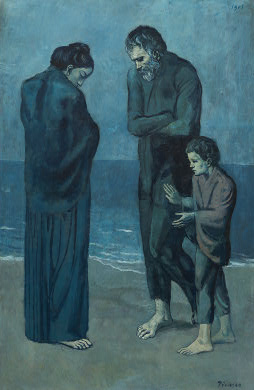
\includegraphics[width=0.3\linewidth]{fig/Poor-nga.jpg} &
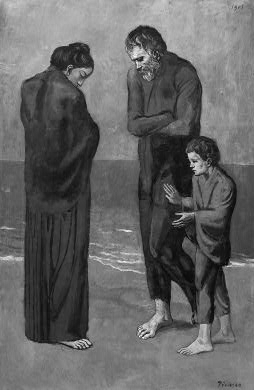
\includegraphics[width=0.3\linewidth]{fig/Poor-nga-sparse_dr.png} & 
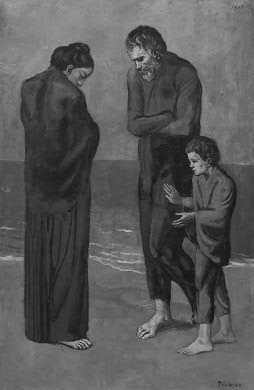
\includegraphics[width=0.3\linewidth]{fig/Poor-nga-rgb2gray.png} \\
(a) The Tragedy & (b) Our result & (c) rgb2gray
\end{tabular} 	
\end{center}
\caption{Emotional impression depicted in various blues is lost after decolorization.}
\label{fig:difficulty}
\end{figure}

As we have discussed in the previous section, 
most of the existing techniques to convert a color image 
into grayscale do attempt to address preserving not only the luminance 
but also the chromatic information. 
However, their formulation often investigates the related features 
either in the original color space or 
in yet another color space of the same dimension. 
In our method, we instead transform the 3-D color space 
into a new feature space of higher-dimensions. 
We achieve this effect by learning an image-dependent dictionary $D$
to account for the important features such as color and saliency distributions.
To go from the original color space to this new space, 
denoted as $F^{|D|} \subseteq \mathbb{R}^{|D|}$, 
without significantly increasing the computational complexity,
we consider a sparse linear model \cite{Seeger08:BIO} over $D$,
and more significantly, 
we show that the underlying relations among the luminance and chromatic features
can be better revealed in $F^{|D|}$. 
Hence, designing a transformation to carry out color conversion 
by preserving the relations there would generally lead to a more effective scheme.

%
\subsection{Overall framework}
\label{sec:framework}
%

The main challenge of decolorization is the loss of visually
meaningful chromatic information, which in certain cases is extremely hard
to maintain after converting to a grayscale image. 
Take, for example, the famous painting ``The Tragedy'' by Pablo Picasso 
shown in Figure~\ref{fig:difficulty}. Without relying parameter hand-tuning,
most of the state-of-the-art techniques or softwares for decolorization 
would not be able to capture the emotional impression depicting by the various blues.
One main reason for the difficulty is that visually meaningful contents
inspired by chromatic stimuli cannot be appropriately represented in a 3-D color space.
And it causes most of the related techniques to fail. 
Nevertheless, as we will describe later, chromatic information of less subtlety
can be more satisfactorily retained in a systematic framework over $F^{|D|}$.

\ignore{
\begin{figure}[t]
\begin{center}
\begin{tabular}{c}
\psfrag{RGB}{{\sssmall RGB}}
\psfrag{linear transformation}{{\sssmall linear projection $P$}}
\psfrag{inner product}{{\sssmall inner product}}
\psfrag{preserving}{{\sssmall preserving}}
\psfrag{grayscale}{{\sssmall grayscale}}
\psfrag{feature space}{{\sssmall feature space}}
\psfrag{F}{{\sssmall $F^{|D|}$}}		
\psfrag{Dictionary}{{\sssmall dictionary $D$}}	
\includegraphics[height=2.0in]{fig/overview.eps}
\end{tabular} 	
\end{center}
\caption{The linear projection $P$ is to preserve the feature relations in $F^{|D|}$.}
\label{fig:overview}
\end{figure}
}

Motivated by the recent success in adopting the sparse linear model
to tackle various vision applications, we propose a decolorization method 
that the formulation is established based on the assumption: 
{\em The luminance and the chromatic features of an image 
are better described in $F^{|D|}$ than in the original color space.}
This is in general true since, contrary to a universal color space, 
$F^{|D|}$ is specifically constructed for each image. 
A sparse linear model can be expressed by

\begin{equation}
\mathbf{x} = D \mathbf{c} + \epsilon
\label{eqn:sparse}
\end{equation}

\noindent where $\epsilon$ is a Gaussian noise, 
and the coefficients in $\mathbf{c}$ are assumed to be i.i.d. 
drawn from a Laplace distribution. 
To perform decolorization, we begin by adaptively learning a dictionary 
from a given color image. 
The resulting dictionary would reasonably encode the {\em principal} luminance 
and chromatic information. 
We further consider the {\em lasso} model \cite{Tibshirani94} of sparse coding
to conveniently locate the mapping from the color space to the feature space 
induced by the dictionary. 
Finally, a closed-form solution to perform dimensionality reduction 
from the new space to the grayscale space is then applied to complete the color conversion.
In Figure~\ref{fig:overview}, we illustrate the whole procedure of our approach.

%
\subsection{Dictionary learning}
\label{sec:dict}
%

Given a color image $I = \{\mathbf{x}_i = (r_i, g_i, b_i)^T\}_{i=1}^n$ of $n$ pixels, 
we apply the image segmentation algorithm by Felzenszwalb and 
Huttenlocher~\cite{Felzenszwalb:2004:EGI} to derive a collection of superpixels, 
and calculate the mean color vector $ \mathbf{m}_j = (r_j, g_j, b_j)^T$ of each segment $j$.
To emphasize those that are visually significant, 
we also compute a saliency map using the method presented in \cite{Goferman10}.
The sum of the saliency values for pixels in segment $j$ is denoted as $s_j$. 
We further assume that $\{ \mathbf{m}_j\}$ is arranged as a sorted list 
in a descending order of $s_j$.

To construct a dictionary $D$ for decolorizing $I$, we need a pool $\Omega$ 
of possible atoms, which are collected by sequentially adding $\mathbf{m}_j$ to the pool,
if it is sufficiently {\em dissimilar} to those already in $\Omega$, \ie,

\begin{equation}
\mathrm{dist}(\mathbf{m}_j, \Omega) = \min\limits_{\mathbf{m}_k \in \Omega} \mathrm{dist}(\mathbf{m}_j, \mathbf{m}_k) < \delta
\label{eqn:delta}
\end{equation}

\noindent where $\delta$ is a parameter, and set to $0.3$ in all our experiments.
Apparently, $\Omega$ is a still a sorted list, 
and indeed a refined set of $\{ \mathbf{m}_j\}$. 
Our criterion for an ideal $D$ is that it should include atoms with large $s_j$, 
and meanwhile each of them should play a significant role in the sparse coding. 
More precisely, suppose we have chosen a subset of atoms from $\Omega$ to yield $D$.
It is thus preferable that the atoms are from the front end of $\Omega$. 
To check whether $D$ is a proper dictionary for sparse coding with respect to $I$,
we solve the following lasso problems:

\begin{equation}
\min\limits_{\mathbf{c}_i} \frac{1}{\alpha^2} \| \mathbf{x}_i - D\mathbf{c}_i \|^2_2 + \frac{1}{\beta} \|\mathbf{c}_i\|_1
\label{eqn:lasso}
\end{equation}

\noindent for all $\mathbf{x}_i \in I$, 
where the two parameters in (\ref{eqn:lasso}) are related by $\alpha^2/\beta = 0.05$
as suggested in \cite{YangYH10}. 
The scatter matrix of $I$ under the mapping $\mathbf{x}_i \mapsto \mathbf{c}_i$ is given by

\begin{equation}
M = \sum\limits_i (\mathbf{c}_i-\bar{\mathbf{c}})(\mathbf{c}_i-\bar{\mathbf{c}})^T
\label{eqn:scatter}
\end{equation}

\noindent where $\bar{\mathbf{c}}$ is the mean of $\{\mathbf{c}_i\}$. 
When $M$ is not full-rank, it implies that there exist {\em non-informative} atoms in $D$,
and they are not used (or rarely used) in performing sparse coding for $I$.
For a color image of a large size, solving (\ref{eqn:lasso}) for all pixels 
is time-consuming. 
In that case, a downsample version of $I$ will instead be considered. 
We describe a practical implementation for learning $D$ in Algorithm~\ref{Alg:dictionary}
that can avoid a naive and time-consuming way of sequentially adding the atoms to construct
$D$ until the condition of full rank is violated.

\begin{algorithm}[tH]
\SetKwInOut{Input}{Input} %
\SetKwInOut{Output}{Output} %
\DontPrintSemicolon %
\SetAlgoLined %
\Input{An image $I=\{\mathbf{x}_i\}$ of tatal saliency value $s$,
a sorted list $P=\{\mathbf{m}_j\}$ with its corresponding $\{s_j\}$,
and a parameter $ r \in (0.5,1]$.}%
\Output{$D$.} %
\BlankLine %
1. $r \leftarrow \min\{r, {\sum_j s_j}/s\}$.\; %
2. Initialize $D$ by selecting the least $k$ atoms from $P$ such that $\sum_{j=1}^k s_j/s \ge r$.\; %
3. $J \leftarrow \mathrm{downsample}(I)$. \; %
4. Solve the lasso problem (\ref{eqn:lasso}) for all $\mathbf{x}_i \in J$. \;%
5. Compute the scatter matrix $M$ as in (\ref{eqn:scatter}).\;%
6. \If{$M$ is not full-rank}{
       Remove the last $k-\mathrm{rank}(M)$ atoms from $D$.\;%
       $k \leftarrow |D|$.\;%
       Repeat steps 4, 5, and 6.\;%
    }{return $D$}
\caption{Learning $D$ for decolorization. \label{Alg:dictionary}}
\end{algorithm}

% advantage higher space without redundancy cf. main-theme vector
% justifications why full-rank , zeros of _ci , unnecessary,


It is insightful to discuss the properties of $D$ in more detail. 
First, observe that the resulting dictionary is established by including 
as many atoms as possible, 
providing it would not break the full-rank condition on the scatter matrix of the sparse coefficient vectors. By enforcing this constraint, 
our method does not introduce extra and unnecessary feature dimensions 
in transforming the color space to the $F^{|D|}$. 
As we will see in the next section, 
this nice property of $D$ is also useful in finding the exact form of 
the linear projection to the grayscale space. 
Second, the atoms of $D$ are {\em representative} as they are considered 
in a descending order of the sum over the saliency values of their respective pixels 
so that each atom corresponds to the mean color vector of 
either a large or a salient segment. 
We also require them to significantly account for the saliency distribution of $I$. 
(See Algorithm~\ref{Alg:dictionary}).

%
\subsection{Grayscale conversion}
\label{sec:grayscale}
%

We are now ready to discuss how to carry out the linear projection 
to convert a color image into grayscale. 
Since we are to preserve the feature relations in $F^{|D|}$ after performing 
linear projection, we consider solving the following optimization problem:

\begin{equation}
\min_{P} \sum_i \sum_j (\mathbf{c}_i - \mathbf{c}_j)^T(P\mathbf{x}_i - P\mathbf{x}_j)
\label{eqn:optimization}
\end{equation}

\noindent where $P$ is a 1-D linear projection (\ie, a $1\times 3$ matrix) 
form the input color space to the grayscale space. 
In solving (\ref{eqn:optimization}), we first need to solve the lasso problem 
defined in (\ref{eqn:lasso}) for all pixels in $I$,
which would be impractical for images of large sizes. 
However, owing to the lasso model (\ref{eqn:lasso}) in linking $\mathbf{x}_i \in I$ 
and its sparse code $\mathbf{c}_i$, a closed-form solution of (\ref{eqn:optimization}) 
derived by Gkioulekas and Zickler \cite{Gkioulekas:2011:DRU} can be directly applied. 
It follows that

\begin{equation}
P = L R = \mathrm{diag}(f(\lambda)) \mathbf{V}^T R
\label{eqn:projection}
\end{equation}
\noindent where
\begin{equation}
f(\lambda) = \left(\frac{4\beta^4\lambda}{\alpha^4+4\beta^2\alpha^2\lambda+4\beta^4\lambda^2}\right)^{1/2}
\label{eqn:f}
\end{equation}
\noindent
and $\lambda$ is the largest eigenvalue of the matrix $D^TD$, 
$\mathbf{V}$ is the corresponding eigenvector, 
$\alpha$ and $\beta$ are the parameters in (\ref{eqn:lasso}), 
and $R$ is a $3 \times 3$ rotation matrix to be decided. 
Recall that the dictionary $D$ is derived by adding the mean vector $\mathbf{m}_j$ 
according to a descending order of saliency values, 
while respecting the full-rank constraint. 
The criterion can help not only avoid introducing unnecessary feature dimensions 
but also measure the {\em goodness} of a rotation matrix. 
To that end, we consider solving

\begin{equation}
\max_{R} \sum\limits_{j=1}^{|D|} \sum\limits_{k=1}^{|D|} s_j (P\mathbf{m}_j - P\mathbf{m}_k)^2 = \sum\limits_{j=1}^{|D|} \sum\limits_{k=1}^{|D|} s_j (LR\mathbf{m}_j - LR\mathbf{m}_k)^2\,.
\label{eqn:rotation}
\end{equation}

The optimization problem (\ref{eqn:rotation}) is to seek for an optimal rotation matrix $R$
such that the saliency features can be preserved after the dimensionality reduction. 
Solving (\ref{eqn:rotation}) is nontrival, and the quality of a local-minimal 
``solution'' heavily depends on the initial guess of $R$. 
We instead ``solve'' (\ref{eqn:rotation}) by uniformly sampling a large number of 
3-D rotation matrices, and adopt the one with the maximal objective value for our use. 
In all our experiments, we generate 100,000 such matrices, and the technique 
empirically achieves better performance than optimizing (\ref{eqn:rotation}) 
using the identity matrix as a starting point.

\section{Experiments}
\label{sec:experiments}

We discuss the benefits and drawbacks of our framework in this section.
In the first place, parameters choosing and tuning are important issues in decolorization.
Experienced users can use proprietary programs such as Adobe Photoshop 
to create their desired grayscale images.
However, such editing is not familiar to amateurs, so an automatic algorithm seeking 
a solution to facilitate this process without users' interference is necessary.
On the other hand, performance is also an important issue. 
Users expect outputs immediately because the baseline algorithm, eg. rgb2gray, 
is really fast to perform the color conversion.
A competitive algorithm should not far from this performance unless it deals with
particular details and makes tremendous different results.
Our algorithm has benefits on tuning parameters and compatible performance.
Moreover, our algorithm maintain the visual appearance in general unless the limited
cases which would be discussed in the end of this section.

\begin{figure}[t]
\begin{center}
\begin{tabular}{ccc}
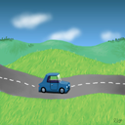
\includegraphics[width=0.27\linewidth]{fig/Voiture.png} &
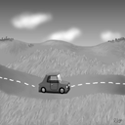
\includegraphics[width=0.27\linewidth]{fig/Voiture-sparse_dr-colorT03_resize01.png} &
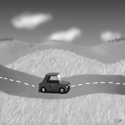
\includegraphics[width=0.27\linewidth]{fig/Voiture-sparse_dr-colorT02_resize01.png} \\
%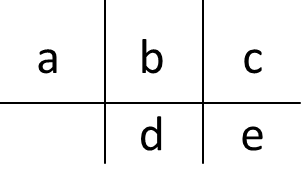
\includegraphics[width=0.10\linewidth]{fig/abcde.png} &

\includegraphics[width=0.27\linewidth]{fig/Voiture-visD-all.png} &

\includegraphics[width=0.27\linewidth]{fig/Voiture-visD-colorT03.png} & 

\includegraphics[width=0.27\linewidth]{fig/Voiture-visD-colorT02.png} \\
\end{tabular}
\caption{
\textbf{Effect of the threshold by choosing different atoms.} 
From left to right, up to down with alphabet order:
(a) original image,
(b) ours with $\delta=0.3$,
(c) ours with $\delta=0.2$,
(d) mean color from the segmentation of original image in saliency descent order,
(e) dictionary with $\delta=0.3$,
(f) dictionary with $\delta=0.2$.
Our algorithm picks atoms follow in saliency descent order. In this case, comparing with
Olive Drab (the third atom of (d)), Sea Green (the forth atom of (e)) is too similar 
under the threshold $\delta=0.3$,
so our algorithm choose Sky Blue under this setting.
When Sea Green is considered as basis, the difference between two similar colors
will be amplified.}
\label{fig:parameters}
\end{center}
\end{figure}

\subsection{Parameters}
\label{sec:parameters}
The main problem of decolorization is complicated parameter setting.
Most of the algorithms need to decide lots of parameters because 
their operators inherently have more complicated function.
For instance, the offset angle of color wheel serves the task of preventing
saliency lost in~\cite{Gooch:2005:CSC,Ancuti:2011:ESG}.
It controls the mapping between chromatic and illuminance differences.
By assigning particular angle, the operators could enhance detail for
color-deficient observers.
While to embedded these kind of parameters in algorithm risk to make unwanted artifact.
In contrast with these methods, we avoid to introduce offset angle and 
utilize some preliminary information to prevent the saliency lost.

Our framework, combining segmentation, saliency map computation, and dimensionality
reduction by sparse model, seems complicated at first glance,
but these factors can be friendly applied with their default setting for most of cases
in our experiments.
The main point in our framework is to construct the dictionary $D$,
and the chief parameter behind this procedure is the color threshold $\delta$.
Our procedure decides whether a color is suitable for adding in the dictionary by
judging if this color exceeds the colors have been collected over the threshold $\delta$.
In our experiment, this factor is reliable only if we have special requirement
to distinguish similar color in grayscale.
Figure~\ref{fig:parameters} illustrates the function of this parameter.
Without notification, we use the default parameter $\delta=0.3$ for all results in
this paper.

%

\begin{figure}[t]
\begin{center}
\begin{tabular}{cccc}

\includegraphics[width=0.2\linewidth]{fig/colorwheel.jpg} &
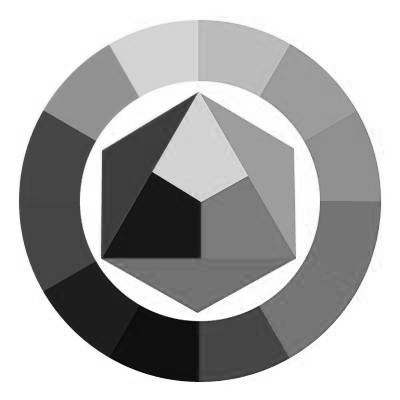
\includegraphics[width=0.2\linewidth]{fig/colorwheel-sparse_dr.png} &

\includegraphics[width=0.2\linewidth]{fig/colorwheel-pca_rgb.png} & 

\includegraphics[width=0.2\linewidth]{fig/colorwheel-pca_lab.png} \\
color & ours & RGB & CIE{\it L*a*b}
\end{tabular}
\caption{
\textbf{Dimensionality reduction on difference spaces.}
The comparison between our method and PCA directly applying on RGB and CIE{\it L*a*b}
demonstrates the sensitivity of PCA on different basis. Our method chooses a reasonable
basis for individual input images.
}\label{fig:PCA}
\end{center}
\end{figure}



\begin{figure}[t]
\begin{center}
\begin{tabular}{ccc}
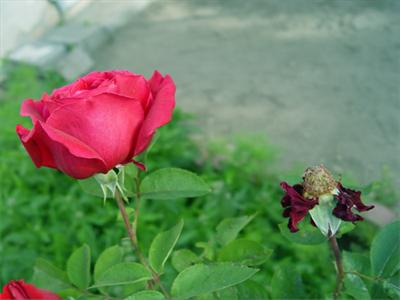
\includegraphics[width=0.3\linewidth]{fig/2_75_75169.png} &
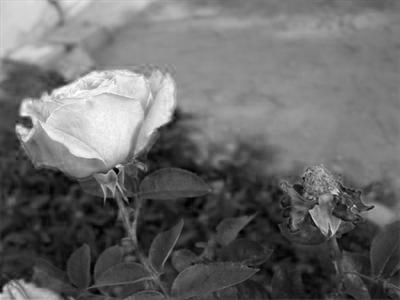
\includegraphics[width=0.3\linewidth]{fig/2_75_75169-sparse_dr.png} & 
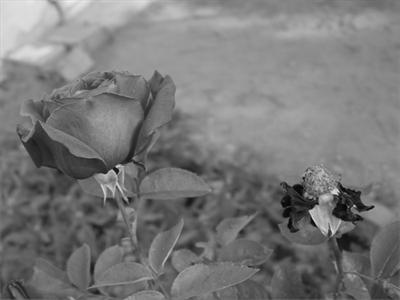
\includegraphics[width=0.3\linewidth]{fig/2_75_75169-rgb2gray.png} \\
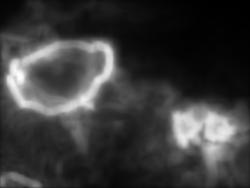
\includegraphics[width=0.3\linewidth]{fig/2_75_75169_SaliencyMap.jpg} &
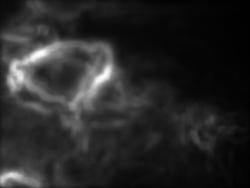
\includegraphics[width=0.3\linewidth]{fig/2_75_75169-sparse_dr_SaliencyMap.jpg} & 
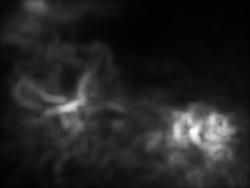
\includegraphics[width=0.3\linewidth]{fig/2_75_75169-rgb2gray_SaliencyMap.jpg} \\
color & ours & rgb2gray \\
\end{tabular}
\caption{
\textbf{Saliency preserving decolorization.}
The first row shows the original color image and three different grayscale images,
and the second row shows the saliency detected by~\protect\cite{Hou:2012:ISH} 
on them. When an unavoidable information loss occurs,
our method prior preserves the saliency on significant regions in grayscale.
In this case, there are two followers in the image, the left one was chose by
purposed algorithm.
}\label{fig:saliency}
\end{center}
\end{figure}

\subsection{Salient object preserving}
\label{sec:saliency}
Our method can be viewed as performing PCA on higher dimensional space
rather than the original color space.
While PCA has been studied for decolorization in~\cite{Gooch:2005:CSC}, the space
of applying such technique was vague and it is worth to discuss herein.
As discussion in~\cite{Gooch:2005:CSC}, PCA is quite sensitive in which computation
takes place. Figure~\ref{fig:PCA} shows that performing PCA on color spaces such as
RGB and CIE{\it L*a*b} have dramatic differences.

The point is our framework effectively chooses specific color codewords, namely basis,
to perform PCA, and the data on the basis reveal a good structure for preserving saliency
after applying dimensionality reduction.
We discuss the property by analyzing the scatter matrix of the data points
and applying saliency detection after decolorzing on these two spaces.

To tell the difference between original color space and the hyperspace,
we first explore the ratio of the largest eigen value $\lambda_1$ over 
the sum of all eigen value on the scatter matrix of the pixels sample from a space, 
denote the ratio by 
$r = \lambda_1 / \sum_i \lambda_i$.
Theoretically, data are easier to be represented in single channel 
by dimensionality reduction with higher $r$. 
We computed the ratio over $24$ color images in the collection of~\cite{Ancuti:2011:ESG}.
The mean of $r$ is equal to $0.8491$ and $0.8169$ on the hyperspace and the original color
space, so the difference is not distinguish at first sight.
However, the salient regions in grayscale 
have obviously different distribution on the two spaces.
Figure~\ref{fig:saliency} demonstrate this observation.
Our algorithm visually preserves the salient region as the original image.
Moreover, we apply saliency detection algorithm on color and grayscale images, and
the results make the differences more definite.

\newcommand{\sfont}{\scriptsize}
\newcommand{\rb}[1]{\raisebox{1.0ex}[0pt]{#1}}
\begin{table}[t]{\tiny
\caption{\textbf{The computation time of a $710\times480$ input image.}} 
\begin{center}{\sfont
\begin{tabular}{|>{\centering}p{1cm}|>{\centering}p{1cm}|>{\centering}p{1cm}|>{\centering}p{1cm}|>{\centering}p{1cm}|>{\centering}p{1.1cm}|p{1cm}<{\centering}|} \hline%
              &             &               &              &              &                  &          \\%
\rb{Method}   &  \rb{Ours}  & \rb{Ancuti11} & \rb{Kim09}   & \rb{Smith08} & \rb{Grundland07} &  \rb{Gooch05} \\ \hline %
              &             &               &              &              &                  &          \\%
\rb{Running}  &  \rb{1 sec} & \rb{1 sec}    & \rb{0.5 sec} & \rb{11 sec}  & \rb{0.1 sec}     &  \rb{5 min}   \\ \hline %
\end{tabular}}
\end{center}
\label{tbl:performance}}
\end{table}

\subsection{Performance}
\label{sec:performance}
The results were generated by a non-optimized MatLab code on a Personal Computer 
with four-core Intel CPU and 16 GB RAM.
The computational time of our algorithm is dominated by solving the lasso problem.
While this step only play the rule of checking the dictionary rank, in other words,
we do not need to solve it for total amounts of the input pixels.
We downsample the image for speeding up the whole procedure.
The performance raise ten times from $10$ to $1$ second on a $710\times480$ image by
reducing the input image to $71\times48$ under our implementation.
By our experiment, sampling on the thumbnail image with approximate thousand of pixels
is enough to present results in our paper.
Table~\ref{tbl:performance} lists the computation time for reference.
To speed up current implementation, parallel computation on lasso and random sampling
of rotation matrix is available without modified the framework.
Other advance approaches such as lasso screening~\cite{Xiang:2011:LSP} are also
encouraged to reduce the computation complexity. 
Since our method performs on the dictionary constructed by superpixels, 
it has very limited memory requirement comparing with 
the pixel-based methods~\cite{Gooch:2005:CSC}.
The typical dictionary size is from $5$ to $7$, depend on the color distribution of 
input image.
Because the size of dictionary is not proportion to image size, 
our method is suitable to scale up for high resolution image.

\section{Results}
\label{sec:results}

\begin{figure*}[t]
\begin{center}
\begin{tabular}{c@{\;}c@{\;}c@{\;}c@{\;}c@{\;}c@{\;}c@{\;}c@{\;}c@{\;}c}

\includegraphics[width=0.10\linewidth]{fig/supp/c07.png} &

\includegraphics[width=0.10\linewidth]{fig/supp/c07-sparse_dr.png} &

\includegraphics[width=0.10\linewidth]{fig/supp/c07-rgb2gray.png} &

\includegraphics[width=0.10\linewidth]{fig/supp/c07-ancuti2011.png} &

\includegraphics[width=0.10\linewidth]{fig/supp/c07-kim2009.png} &

\includegraphics[width=0.10\linewidth]{fig/supp/c07-smith2008.png} &

\includegraphics[width=0.10\linewidth]{fig/supp/c07-pr2006.png} &

\includegraphics[width=0.10\linewidth]{fig/supp/c07-gooch2005.png} &

\includegraphics[width=0.10\linewidth]{fig/supp/c07-rasche2005.png} \\

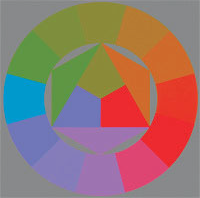
\includegraphics[width=0.10\linewidth]{fig/supp/c08.png} &
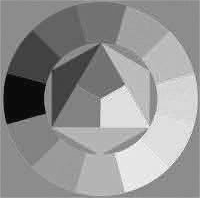
\includegraphics[width=0.10\linewidth]{fig/supp/c08-sparse_dr.png} &

\includegraphics[width=0.10\linewidth]{fig/supp/c08-rgb2gray.png} &
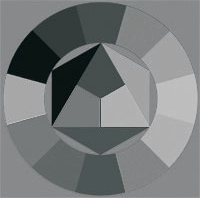
\includegraphics[width=0.10\linewidth]{fig/supp/c08-ancuti2011.png} &

\includegraphics[width=0.10\linewidth]{fig/supp/c08-kim2009.png} &

\includegraphics[width=0.10\linewidth]{fig/supp/c08-smith2008.png} &

\includegraphics[width=0.10\linewidth]{fig/supp/c08-pr2006.png} &

\includegraphics[width=0.10\linewidth]{fig/supp/c08-gooch2005.png} &
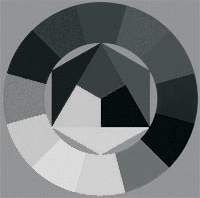
\includegraphics[width=0.10\linewidth]{fig/supp/c08-rasche2005.png} \\

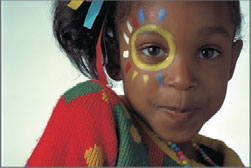
\includegraphics[width=0.10\linewidth]{fig/supp/c11.png} &
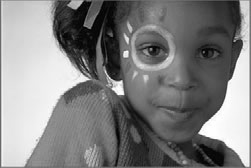
\includegraphics[width=0.10\linewidth]{fig/supp/c11-sparse_dr.png} &
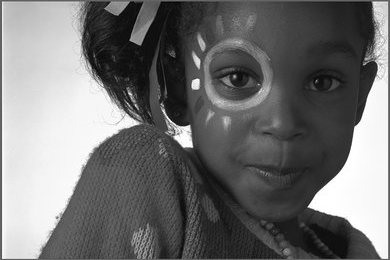
\includegraphics[width=0.10\linewidth]{fig/supp/c11-rgb2gray.png} &
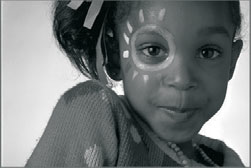
\includegraphics[width=0.10\linewidth]{fig/supp/c11-ancuti2011.png} &
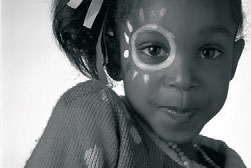
\includegraphics[width=0.10\linewidth]{fig/supp/c11-kim2009.png} &
\includegraphics[width=0.10\linewidth]{fig/supp/c11-smith2008.png} &
\includegraphics[width=0.10\linewidth]{fig/supp/c11-pr2006.png} &
\includegraphics[width=0.10\linewidth]{fig/supp/c11-gooch2005.png} &
\includegraphics[width=0.10\linewidth]{fig/supp/c11-rasche2005.png} \\

\includegraphics[width=0.10\linewidth]{fig/supp/c23.png} &
\includegraphics[width=0.10\linewidth]{fig/supp/c23-sparse_dr.png} &
\includegraphics[width=0.10\linewidth]{fig/supp/c23-rgb2gray.png} &
\includegraphics[width=0.10\linewidth]{fig/supp/c23-ancuti2011.png} &
\includegraphics[width=0.10\linewidth]{fig/supp/c23-kim2009.png} &
\includegraphics[width=0.10\linewidth]{fig/supp/c23-smith2008.png} &
\includegraphics[width=0.10\linewidth]{fig/supp/c23-pr2006.png} &
\includegraphics[width=0.10\linewidth]{fig/supp/c23-gooch2005.png} &
\includegraphics[width=0.10\linewidth]{fig/supp/c23-rasche2005.png} \\

\includegraphics[width=0.10\linewidth]{fig/supp/c24.png} &
\includegraphics[width=0.10\linewidth]{fig/supp/c24-sparse_dr.png} &
\includegraphics[width=0.10\linewidth]{fig/supp/c24-rgb2gray.png} &
\includegraphics[width=0.10\linewidth]{fig/supp/c24-ancuti2011.png} &
\includegraphics[width=0.10\linewidth]{fig/supp/c24-kim2009.png} &
\includegraphics[width=0.10\linewidth]{fig/supp/c24-smith2008.png} &
\includegraphics[width=0.10\linewidth]{fig/supp/c24-pr2006.png} &
\includegraphics[width=0.10\linewidth]{fig/supp/c24-gooch2005.png} &
\includegraphics[width=0.10\linewidth]{fig/supp/c24-rasche2005.png} \\

color & ours & rgb2gray & Ancuti11 & Kim09 & Smith08 & \shortcite{Grundland:2007:DFC} & Gooch05 & Rasche05
\end{tabular}
\caption{
\textbf{Comparison with previous methods.}
From left to right: original color images, ours with default setting $\delta=20$ and $vw=0.1$,
standard rgb2gray in MatLab, Ancuti~\etal~\protect\shortcite{Ancuti:2011:ESG},
Kim~\etal~\protect\shortcite{Kim:2009:RCV}, 
Smith~\etal~\protect\shortcite{Smith:2008:AGA}, 
Grundland and Dodgson~\protect\shortcite{Grundland:2007:DFC}, 
Gooch~\etal~\protect\shortcite{Gooch:2005:CSC},
and Rasche~\etal~\protect\shortcite{Rasche:2005:RIG}.
From top to down: Three cases demonstrate that, comparing with previous methods, 
our algorithm maintain the visual appearance with
perceptually preserving the saliency, keeping the order in chromatics, and without
over enriching the contrast.
}
\label{fig:comparison}
\end{center}
\end{figure*}

We compare the results between our algorithm and previous decolorziation
methods~\cite{Ancuti:2011:ESG,Kim:2009:RCV,Smith:2008:AGA,Grundland:2007:DFC,Rasche:2005:DPR,Gooch:2005:CSC} in Figure~\ref{fig:comparison}.
With a suitable feature transform, we preserve contrast and saliency without suffering
from isoluminants in the input image.
As a global color mapping, our algorithm avoid to create artifacts such as halos, noise
or broken segments in pixel-based 
computation~\cite{Bala:2004:SCT,Gooch:2005:CSC,Rasche:2005:RIG}.
In contrast with other global methods, we straightly preserve the most salient region
in the images to exploit the power of linear operator as the demonstration in
Figure~\ref{fig:saliency}.
Comparing with the most recent work by Ancuti~\etal~\cite{Ancuti:2011:ESG},
both of our works focusing on saliency preserving transformation,
our method further avoid to map different chromatics into the same luminance
and boost the contrast more as the demonstration in Figure~\ref{fig:comparison}.

\subsection{Contrast enhancement imaging}

\begin{figure*}[t]
\begin{center}
\begin{tabular}{ccccc}
\includegraphics[width=0.18\linewidth]{fig/i02.png} &
\includegraphics[width=0.18\linewidth]{fig/i02-rgb2gray.png} &
\includegraphics[width=0.18\linewidth]{fig/i02-sparse_dr.png} &
\includegraphics[width=0.18\linewidth]{fig/i02-enhance.png} &
\includegraphics[width=0.18\linewidth]{fig/i02-iccp2012.png} \\
\includegraphics[width=0.18\linewidth]{fig/i04.png} &
\includegraphics[width=0.18\linewidth]{fig/i04-rgb2gray.png} &
\includegraphics[width=0.18\linewidth]{fig/i04-sparse_dr.png} &
\includegraphics[width=0.18\linewidth]{fig/i04-enhance.png} &
\includegraphics[width=0.18\linewidth]{fig/i04-iccp2012.png} \\
color & rgb2gray & ours & ours+color & Lu12
%
\end{tabular}
\caption{
\textbf{Salient region enhancement.}
From left to right: original color image, rgb2gray, our grayscale image, our enhancing
image, Lu~\etal's image~\protect\cite{Lu:2012:CPD}.
Our graysacle image with enhancing contrast can use to boost the contrast and
relight the region of interest.
}
\label{fig:enhancing}
\end{center}
\end{figure*}

\begin{figure*}[t]
\begin{center}
\begin{tabular}{cccc}
\includegraphics[width=0.2\linewidth]{fig/r08.png} &
\includegraphics[width=0.2\linewidth]{fig/r08-rgb2gray.png} &
\includegraphics[width=0.2\linewidth]{fig/r08-sparse_dr.png} &
\includegraphics[width=0.2\linewidth]{fig/r08-enhance.png} \\
color & rgb2gray & ours & ours+color
%
\end{tabular}
\caption{
\textbf{Image detail enhancement.}
Our grayscale image makes original image sharpen.
}
\label{fig:dehazing}
\end{center}
\end{figure*}

To enrich the contrast of the original image, we substitute the {\it L} of {\it L*a*b}
by our salient-enhancing monochrome image. Comparing with Ju~\etal~\cite{Lu:2012:CPD},
our method prefers to map high salient region into bright luminance. 
Therefore, the enhancing image not only increase the contrast but also 
light up the particular region of interest as showing in Figure~\ref{fig:enhancing}.

The enhancing contrast image can help to dehaze with the same strategy. 
Figure~\ref{fig:dehazing} demonstrates the dehazed imaging obtained by our method.

% weakness of our method
\ignore{
\begin{figure}[t]
\begin{center}
\begin{tabular}{cccc}
\includegraphics[width=0.2\linewidth]{fig/collect.jpg} &
\includegraphics[width=0.2\linewidth]{fig/collect-sortseg.png} &
\includegraphics[width=0.2\linewidth]{fig/collect-sparse_dr.png} &
\includegraphics[width=0.2\linewidth]{fig/collect-rgb2gray.png} \\
color & importance map & ours & rgb2gray
%
\end{tabular}
\caption{
\textbf{Situation with multiple salient subjects.}
Our framework compute the importance of superpixels as the hint of decolorization.
As second column present, more lighter the map is, more salient of that region.
The result distinguishes the color between the flower and background, but ignore
other subjects which might be more significant in other viewers observation.
}
\label{fig:collect}
\end{center}
\end{figure}
%
\begin{figure}[t]
\begin{center}
\begin{tabular}{cccc}
\includegraphics[width=0.2\linewidth]{fig/c04.png} &
\includegraphics[width=0.2\linewidth]{fig/c04-seg.png} &
\includegraphics[width=0.2\linewidth]{fig/c04-sparse_dr.png} &
\includegraphics[width=0.2\linewidth]{fig/c04-rgb2gray.png} \\
color & segmentation & ours & rgb2gray
%
\end{tabular}
\caption{
\textbf{Situation with failure of segmentation.}
Using default parameters suggested in~\protect\cite{Felzenszwalb:2004:EGI},
the segmentation has a flaw in the boundary between the purple ball and the table.
It makes an incorrect codeword due to the color distortion from purple to imperial blue.
}
\label{fig:segmentation}
\end{center}
\end{figure}
%
Our framework relies on saliency map and region segmentation.
This dependency limits our framework in some cases.
First, since we only focus on the most salient subject in the image, 
our algorithm fail to handle the images with multiple salient region.
The problem may cause by noises which effected the salient estimation.
For example, specular reflection or the stain on the camera lens may form
an unwanted segments.
Alternate the detectors, such as Itti~\etal's~\cite{Itti:1998:AMS} and 
Hou~\etal's~\cite{Hou:2012:ISH}, might help for generating different
salient distribution.
However, salient region specific to different people, and there were no
existed methods have completed solved this problem.
Figure~\ref{fig:collect} shows that there are various subjects in the input canvas.
Second, failure segmentation would distort the codewords of dictionary.
It would effect the decolorization because the optimization in (\ref{eqn:optimization})
is not going to process for the actual distribution of the input image.
Figure~\ref{fig:segmentation} shows this case.
}


{\small
\bibliographystyle{ieee}
\bibliography{egbib}
}

\end{document}
